\chapter{Applying Machine Learning}
In this chapter we give the theory behind the three machine learning techniques that were used in our models to characterise and determine trustworthiness. These are Logistic Regression (LR), Support Vector Machines (SVM) and Random Forests (RM). The reasons behind this are detailed in the following sections, however Figure 5.1 below gives an overview of the performance of each of these models and some of the others.                                                          
\begin{figure}[hb]
  \centering
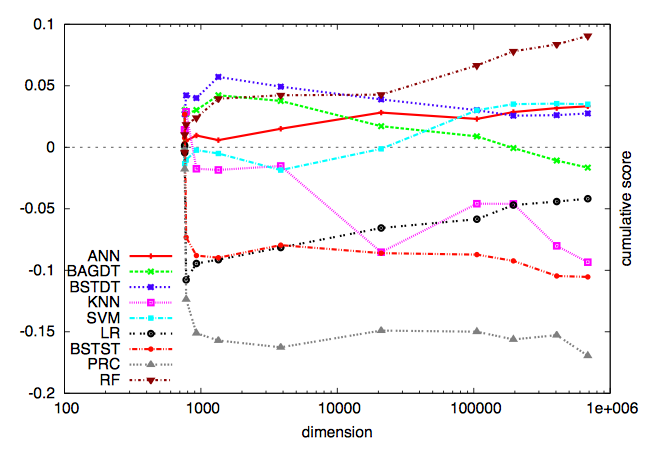
\includegraphics[width=13cm]{MachineLearningModels}
  \caption[Comparison of Machine Learning Models]
   {ANN = Artificial Neural Networks, BAGDT = Bagged Decision Trees, BSTDT = Boosted Trees, KNN = K nearest neighbour, SVM = Support Vector Machines, LR = Logistic Regression, BSTST = Boosted Stumps, PRC = Perceptrons, RF = Random Forests. Cumulative standardised scores of each Machine Learning algorithm as a function of the dimension. (Caruana et al. 2006) }
\end{figure}
\section{Problem Structure}
In this section, we briefly give the problem, the structure of our data and the Twitter features selected to apply Machine Learning. \\*\\*
$\mathbf{Problem}$ : Determining the Trust Worthiness of tweets posted on Twitter.\\*\\*
$\mathbf{Structure}$ : Our data is a collection of $x$ and $y$ data points where $x_i$ is a $d$ dimensional vector and $y$ is a True or False classification\\*
\centerline{$D = ((x_1,y_1),..,(x_n,y_n)) , x_i \in \mathbb{R}^d$  and  $y_i \in {0,1}$}\\*\\*
$\mathbf{Input}$ : $x_1$ = FrequencyOfTweets, $x_2$ = FavouriteCount, $x_3$ = RetweetCount, $x_4$ = InReplyToStatusID, $x_5$ = InReplyToUserID, $x_6$ = Hashtags, $x_7$ = UserMentionID, $x_8$ = URL, $x_9$ = MediaURL, $x_{10}$ = MediaType, $x_{11}$ = PossiblySensitive, $x_{12}$ = Language, $x_{13}$ = TweetLength , $x_{14}$ = Location, $x_{15}$ = Description $x_{16}$ = UserAccountURL, $x_{17}$ = Protected, $x_{18}$ = FollowersCount, $x_{19}$ = FriendsCount, $x_{20}$ = ListedCount, $x_{21}$ = FavouritesCount, $x_{22}$ = Verified, $x_{23}$ = GeoEnabled, $x_{24}$ = StatusesCount, $x_{25}$ = ProfileBackgroundImageURL, $x_{26}$ = ProfileUseBackgroundImage, $x_{27}$ = DefaultProfile, $x_{28}$ = IsItARetweet, $x_{29}$ =  NumberOfSmilies, $x_{30}$ = TweetEmotion, $x_{30}$ = WronglyUsedKeyWords\\*\\*
$\mathbf{System}$ $\mathbf{Specification}$ : Please refer to the Appendix for details of our system as well as the libraries used for training. 
\newpage

\section{Logisitc Regression}
\subsection{Background }
Logistic Regression (LR) is a widely used and important Linear Machine Learning model. By linear we mean that it takes inputs and computes a signal that is a linear combination of the inputs with weights. LR is essentially a probabilistic classification algorithm and it builds the foundation for more complex methods like Neural Networks \cite{40}. This can be used for binary classification and can be extended to multi class classification, however in this section we will specifically look at the algorithm for binary classification. The number of parameters used in LR are also comparatively small, in that, if the dimensions increase the parameters only linearly increase. This could also be easily extended to a multi-class classification. These are some of the reasons for choosing Logistic Regression as one of our models. The only foreseeable drawback is that the performance is not necessarily as good as some of the best performing methods such as Random Forests, Boosted Methods and Support Vector Machines. This however, greatly depends on the nature of the problem and from what we can see this has performed quite well for our problem. 

\subsection{Algorithm}

$\mathbf{Model}$ :  Logistic Regression is a discriminative model and we are aiming to model the probability that a tweet is trustworthy, given some data about it. We write $y_i$ as a Bernouli Random variable with probability $\sigma(w^Tx_i)$ where each of the $y_i$'s are independent. The $w$ here is the parameter and the $x_i$ are fixed and non random. We give weights to each of the variables to get a linear combination. \\*
\centerline{$w_0 + w_1x_1 + w_2x_2 + ... + w_ix_i = w^Tx$ where $x = (1,x_1,x_2,x_3)$} \\*
Here the coefficient $w$ tells us something about how the individual variables are affecting the probability. For instance if $w$ is negative then the probability decreases when the variable increases in value and vice versa. The coefficients also tell us which variables are more influential than the others. A large coefficient regardless of whether it is positive or negative influences the decision more thanks a small coefficient. \\*\\*
\noindent
Let us say that the probability of the the tweet being trustworthy is $P$. Then the probability of the tweet not being trustworthy is $1-P$. The odds ratio then is:$\frac{P}{1 - P}$ \cite{41}\\*\\*
\begin{gather}
\ln (\frac{P}{1 - P}) = w^Tx\\
\frac{P}{1 - P}  = e^{w^Tx} \\
P = (1 - P)\times e^{w^Tx} \\
P = e^{w^Tx} - P\times e^{w^Tx} \\
P + P\times e^{w^Tx} = e^{w^Tx} \\
P(1 + e^{w^Tx}) = e^{w^Tx} \\
P = \frac{e^{w^Tx}}{1 + e^{w^Tx}} \\
P = \frac{1 }{1 + e^{-w^Tx}} (R.H.S \times e^{-w^Tx})
\end{gather}\\*\\*
\noindent
In (5.7) R.H.S if $e^{w^Tx} \to+\infty$, the numerator in this formula below will be very huge and so will the denominator and the ratio will $\approx$ 1. If $e^{w^Tx} \to-\infty$ both numerator and denominator would be very small and $\approx$ 0. If $e^{w^Tx}$ is 0 then $\sigma(e^{w^Tx})$ = 1/2 \\* \\*
\begin{figure}[!h]
 \centering
  \caption[Logistic Regression]
  {Logistic Regression}
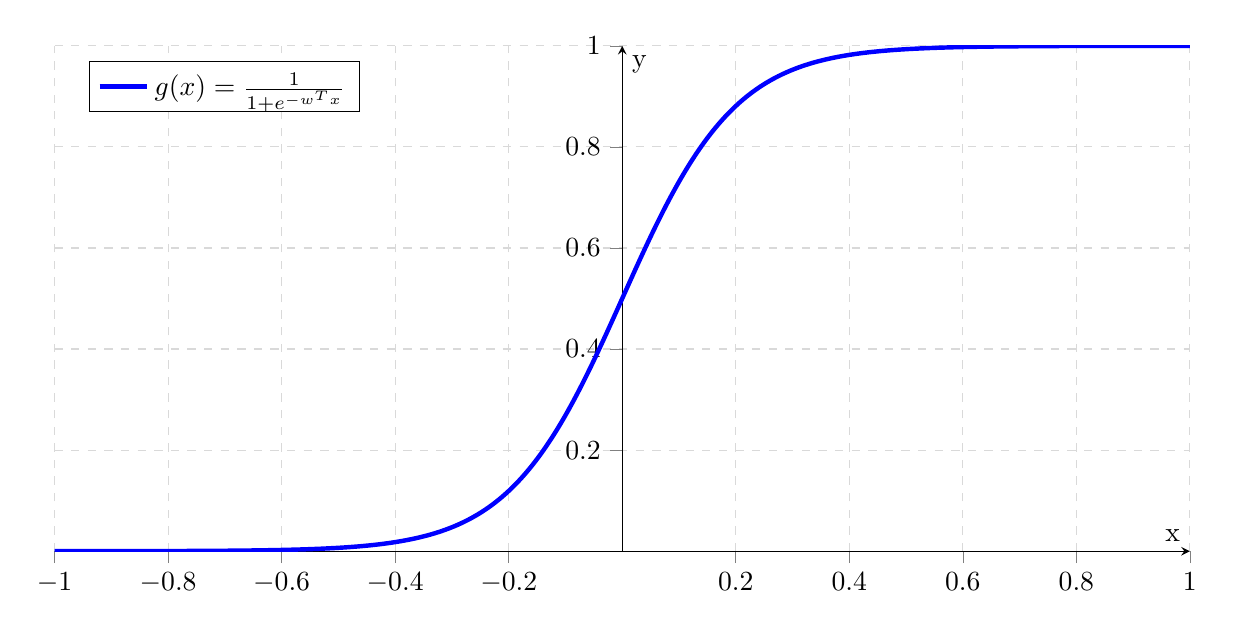
\begin{tikzpicture}
    \begin{axis}[
    	legend pos=north west,
        axis x line=middle,
        axis y line=middle,
        grid = major,
        width=16cm,
        height=8cm,
        grid style={dashed, gray!30},
        xmin=-1,     % start the diagram at this x-coordinate
        xmax= 1,    % end   the diagram at this x-coordinate
        ymin= 0,     % start the diagram at this y-coordinate
        ymax= 1,   % end   the diagram at this y-coordinate
        %axis background/.style={fill=white},
        xlabel=x,
        ylabel=y,
        tick align=outside,
        enlargelimits=false]
      % plot the stirling-formulae
      \addplot[domain=-1:1, blue, ultra thick,samples=500] {1/(1+exp(-10*x))}; 
      \addlegendentry{$g(x)=\frac{1}{1+e^{-w^Tx}}$}
    \end{axis} 
\end{tikzpicture}
\end{figure}\\*\\*
\newpage
\noindent
$\emph{Maximum Likelihood Estimate (MLE)}$ : The Logistic Regression algorithm learns weights so that it can maximise the likelihood of the data. For more detailed explanation please refer to \cite{15}. 
$$L(\vec w) = \sum_{i=1}^{n}\log g(y_iz_i),$$ 
Where $z_i = \sideset{}{_k}\sum w_kx_{ik}$. Note : $1 - g(x) = g(-x)$\\*
The MLE in sklearn\footnote{\url{http://scikit-learn.org}} uses a regularisation parameter. Hence 
$$L = - \sum_{i=1}^{n}\log g(y_iz_i) + \frac{C}{2}\sum_{k=1}^{l} w_k^2$$

\subsection{Application}
The details of the experiment are explained in the next chapter, however here we briefly address some of the points. We first split the data into training and test data sets and then transform the data such that the feature values are normalised. We then pass the training dataset with the features mentioned in section 5.1 into our Logistic Regression model. Once we train this data we then pass the test data into the model to classify and check the accuracy and other measures of this classification. We improve the correctness of this prediction by changing the regularisation parameter to avoid overfitting. 


\newpage
\section{Support Vector Machines}

\subsection{Background}
Support Vector Machines (SVM) is arguably one of the most popular supervised classification methods to date in Machine Learning \cite{31}. It is a linear machine model and the design is greatly influenced by vectors which are closest to the separating hyper plane. The reasons for choosing SVM was because they are effective in high dimensional spaces and use a subset of the training points in the decision function (called support vectors) so it is memory efficient \cite{31}. It is also versatile, in that different kernel functions can be specified for the decision functions. For instance we have used the `Radial Basis Function' kernel\footnote{$\exp(\frac{-\parallel x - x \parallel^2_2}{2\sigma^2})$,  where $\parallel x - x \parallel^2_2$ can be recognised as the squared euclidean distance between two feature vectors and $\sigma$ is a free parameter \cite{33}} and the Polynomial Kernel function\footnote{$K(x,y) = (x^Ty + c)^d$ where $x$ and $y$ are vectors and $c$ is a constant \cite{35}}. The disadvantage with SVM is that the probabilities are calculated using an expensive five-fold cross validation. Moreover if the features : data sample ratio is not fairly low then it may give poor performance. 
\subsection{Algorithm}
We have a two class problem, that is Trustworthy tweets and Untrustworthy tweets. We then have an input feature vector, $\vec x$ which we need to classify as belonging to the Trustworthy class or Untrustworthy Class.  We have a linear discriminant function : 
$$f(x) = w^Tx + b$$
\noindent
Depending on our feature space, this linear equation would be a straight line, plane or hyperplane for two, three or multidimensional feature spaces respectively. The $w$ is a vector which is perpendicular to the hyperplane and it represents the orientation of the hyper plane in our D-dimensional space where D is the dimensionality of the feature vector. The term `b' which is known as a bias term, represents the position of the hyper plane in the D-Dimensional space. In our problem, for every feature vector $\vec x$ we need to compute f(x) and if it falls on the positive side of the hyper plane then we have the following equation satisfied : 
\begin{gather}
f(x) = w^Tx + b > 0 \implies x \in \textup{Trustworthy}
\end{gather}
If it falls on the negative side of the hyper plane we have 
\begin{gather}
f(x) = w^Tx + b < 0 \implies x \in \textup{UnTrustworthy}
\end{gather}
If it falls on the plane we have this : 
\begin{gather}
f(x) = w^Tx + b = 0
\end{gather}
We need to find the $w$ and $b$ such that these values can be used in $f(x)$ to find the separating hyperplane. Hence we train such that for every training sample which belongs to the class `Trustworthy' we start with an initial value for $w$ and $b$ and we check if $f(x)$ is actually greater than 0. If it is not greater than 0 we adjust $w$ and $b$ such that the orientation and position of the hyperplane is shifted till a point where the data point is classified on the positive side of the hyper plane. Likewise we work out a similar procedure for `Untrustworthy tweets'. Let us look at the simple graph below : \\*

\begin{filecontents*}{SVMPlot.csv}
x,y,label
2,2,a
1,4,a
4,3,a
6,5,b
8,7,b
7,9,b
\end{filecontents*}
\begin{tikzpicture}
\begin{axis}
 legend pos=center,
        axis x line=middle,
        axis y line=middle,
        grid = major,
        width=16cm,
        height=6cm,
\addplot [
        % clickable coords={\thisrow{label}},
        scatter/classes={
            a={mark=square*,green},%
            b={mark=square*,red},%
            c={mark=o,draw=black,fill=black}%
        },
        scatter,only marks,
        scatter src=explicit symbolic]
	table [x=x,y=y,meta=label, col sep=comma]
            {SVMPlot.csv};
    \legend{Trustworthy,Untrustworthy}
\end{axis}
\end{tikzpicture}
\begin{gather}
w.x + \frac{b}{\parallel w \parallel} = d
\end{gather}

\noindent
Support vectors are the vectors that are closest to the hyperplane. So in the diagram above every vector that has a distance $d_{min}$ from the hyperplane is a support vector. Our goal in SVM for the hyperplane is to make sure the margin between the data points and the separating planes are as large as possible. Since generally if the margin is larger the generalisation error of the classifier will be lower. If we look at equation(5.12) we would want to maximise $d$ and this can be achieved by minimising $\mid w \mid$ and maximising bias $b$. 
In order to understand which combinations of $w$'s to use to arrive at the best possible margin we need to maximise the margin ($\frac {1}{\parallel w \parallel}$) subject to the fact that for the nearest point which would have the smallest value of $\mid w^Tx_n + b \mid$ = 1. We scale the value of $w$ to make the equation 1. To optimise this we use Lagrange multipliers\footnote{Find the min or max extremes of a function which also contains constraints \cite{32}} with KKT\footnote{Karush-Kuhn-Tucker Conditions \cite{32}} conditions for our constraints; Refer \cite{32} for more information on KKT conditions. 

\newpage
\section{Random Forests}
\subsection{Background}
Decision Tree Learning uses decision trees as a predictive model which maps observations about an item to conclusions about the items target value \cite{42}. These Decision Trees are easily understood by humans, very compact and handles missing and categorical data very well and can handle large non-linear boundaries between groups. However despite all these advantages of trees, we may not find the best tree and there are times when they are not as accurate as SVMs and other state of the art predictors. The solution for this was to use a collection of trees and is termed Random Forests.\\*\\* 
Random Forest is used for prediction, of categorical and continuous data. This method is based on Trees and is fairly simplistic, yet one of the more powerful Machine Learning models. We can see this from the performance of Random Forests in figure 5.1, where Random Forests ranks seconded topped only by Boosted Decision Trees. Random Forests (Breiman, 2001) work as a huge collection of non-correlated decision trees and it is a technique based on bagging.\footnote{Bagging or bootstrap aggregation is a technique for reducing the variance of an estimated prediction function \cite{30}}
\subsection{Algorithm}
\begin{algorithm}[h!]
  \caption{Random Forests, adapted from Trevor et al. \cite{3}}
  \begin{algorithmic}[1]
  \State Observed Data Points D = [($x_i$,$y_i$),$\hdots$,($x_n$,$y_n$)]. 
  \For{i=1 to B}\Comment{B is some number of trees}
  \State (i)Chose a bootstrap sample from $D$, called $D_i$ of size N from the 
  \State  training data.
  \State (ii)Using $D_i$ we construct a Random Forest Tree $T_i$, by re-cursively repeating
  \State  the following steps for each terminal node of the tree, until a minimum node 
  \State  size $n_{min}$ is achieved.
  \While{MinNode != $n_{min}$}
  \State At each node, chose a random subset $m$ of features from the $p$ variables
  \State (We only consider splitting on those features)
  \State Select the best variable/split-point among the m
  \State Split the node into two daughter nodes
  \EndWhile
   \EndFor
   \State We output the collection of trees $\{T_b\}_1^B$
  \end{algorithmic}
\end{algorithm}
Classification: Let $C_b(x)$ be the class prediction of the $b^th$ random-forest
tree. Then $C_{rf}^B(x)$ = majority vote $\{C_b(x)\}^B_1$.

\subsection{Application}
Below we have a Matrix of training samples with their classifiers. \\*\\*
$\textup{Data Set }= \begin{bmatrix}
\textup{ FrequencyOfTweets} & \textup{FavouriteCount} & \textup{RetweetCount} \\
12 & 4 & 6  \\
2 & 0  & 1 \\
\vdots & \vdots & \vdots \\
1 & 2 & 6  \\
5 & 7  & 10
\end{bmatrix}$
$\begin{bmatrix}
\textup{Classifier } \\
\textup{TrustWorthy } \\
\textup{UntrustWorthy} \\
\vdots \\
\textup{UntrustWorthy} \\
\textup{TrustWorthy } 
\end{bmatrix}$\\*\\*
From the above sample set and we create many random combinations of sub sets with randomly picked values from the above main set. For Eg., \\*

$\textup{Data Set 1 }= \begin{bmatrix}
12 & 4 & 6  \\
22 & 10  & 11 \\
\vdots & \vdots & \vdots \\
1 & 2 & 6  \\
15 & 27  & 10
\end{bmatrix}$
$\begin{bmatrix}
\textup{1} \\
\textup{1} \\
\vdots \\
\textup{0} \\
\textup{1} 
\end{bmatrix} \Longrightarrow \textup{Decision Tree 1} $ \\*
$\textup{Data Set 2 }= \begin{bmatrix}
14 & 14 & 6  \\
2 & 0  & 11 \\
\vdots & \vdots & \vdots \\
11 & 0 & 6  \\
5 & 7  & 1
\end{bmatrix}$
$\begin{bmatrix}
\textup{0} \\
\textup{1} \\
\vdots \\
\textup{0} \\
\textup{0} 
\end{bmatrix}  \Longrightarrow \textup{Decision Tree 2}$
\\*\\*\\*
$\textup{Data Set N }= \begin{bmatrix}
17 & 34 & 6  \\
2 & 1  & 1 \\
\vdots & \vdots & \vdots \\
1 & 2 & 6  \\
15 & 7  & 10
\end{bmatrix}$
$\begin{bmatrix}
\textup{1} \\
\textup{0} \\
\vdots \\
\textup{0} \\
\textup{1} 
\end{bmatrix}  \Longrightarrow \textup{Decision Tree N}$
\\*\\*
We now have many decision trees, each with different variations of the classifications and we use all these decision trees to create a ranking of classifiers. For Classification, each tree would provide a class vote and the final classification is based on majority vote. 
\newpage












































